\chapter{Physikalische Aspekte der Schwarmintelligenz am Beispiel von Reglern}

\section{Regler - auch sie sind erklärbar...}

%Inhalt hauptsächlich von http://miris.informatik.tu-ilmenau.de/~koenig/monist/applets/html/PID-Controller.html; beste gefundene Quelle zur Erklärung eines Reglers
Ein Regler hat die Aufgabe, eine Größe, nennen wir sie Größe 1, an die Größe 2 anzupassen. Die Größe 1 ist also der Istwert, der auch als Regelgröße bezeichnet wird und die Größe 2 ist der Sollwert, der auch den Namen Führungsgröße trägt. 
\\Um den Istwert an den Sollwert anzugleichen, vergleicht eine Messeinrichtung die beiden Größen und bildet die Differenz. Diese wird als Regelabweichung bezeichnet, bildet das Eingangssignal für den Regler und wird durch diesen beeinflusst. Das Ausgangssignal des Reglers ist die Stellgröße, quasi der Wert, der bei Größe 1 verändert werden muss, um sie an die Größe 2 anzupassen.\\
\\
Zusammengefasst sind also vier Größen bei einem Regler wichtig:
\begin{itemize}
\item Istwert bzw. Regelgröße
\item Sollwert bzw. Führungsgröße
\item Differenz bzw. Regelabweichung
\item Stellgröße
\end{itemize}
In Abbildung \ref{fig:Bild1} ist das Prinzip eines Reglers nochmals anhand eines Schaltplans aufgeführt. 

%Bild erstellt nach Vorlage von http://miris.informatik.tu-ilmenau.de/~koenig/monist/applets/html/PID-Controller.html
\begin{figure}[htb]
\centering 
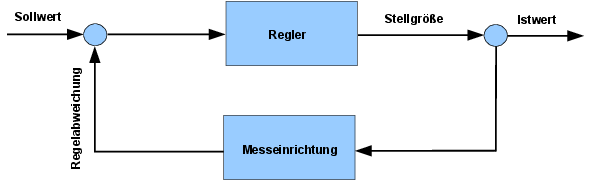
\includegraphics[width=1.05\textwidth]{images/Bild1} 
\vspace{0.2cm}
\caption{Schaltbild eines Reglers.}
\label{fig:Bild1}
\end{figure} 


\section{Der CD-Player - ein Beispiel für einen Regelkreis}
Der CD-Player, dessen Aufbau in Abbildung \ref{fig:Bild2} zu sehen ist, ist ein uns allen bekanntes Beispiel für einen Regelkreis. Die CD-Scheibe liegt auf einem Spindelmotor, dieser rotiert und versetzt die CD in Bewegung. Die Informationen sind auf der CD in Form von "`Pits"' gespeichert, die von einem Laser bestrahlt werden. Das Licht wird an den Pits reflektiert und überlagert sich mit dem restlichen Licht. Die Informationen der CD können mit Hilfe von Photodioden ausgelesen werden, die die Hell-Dunkel-Signale, die durch die Interferenz entstehen, empfangen. 
\\Doch es kann sein, dass die CD beispielsweise axiale Ungenauigkeiten besitzt, dadurch könnte die Übertragung an die Photodioden, die durch eine Linse erfolgen, gestört werden. Hier kommt nun der Regelkreis ins Spiel, der die Aufgabe hat, die Linse mit einer ausreichenden Präzision zu halten, sodass die Übertragung zu den Photodioden und damit das Auslesen der Pits nicht gestört wird.\\
Der CD-Regelkreis misst die Regelabweichungen (den Fokus $r_y$ und die Spurnachführung $r_x$) mit Hilfe der Photodioden, diese bilden das Eingangssignal für den Regler. Das Ausgangssignal sind die Stellgrößen $u_x$ und $u_y$. Um diese muss sich die Linse in x- und y-Richtung bewegen, um ein stabiles Auslesen der Pits zu ermöglichen. 
%Quelle von Bild muss noch angegeben werden; aus Datei, die Christoph Fangohr geschickt hat
\begin{figure}[H]
\centering 
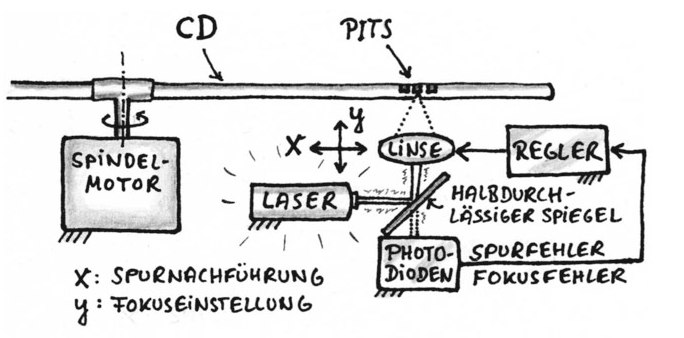
\includegraphics[width=1.05\textwidth]{images/Bild2} 
\vspace{0.2cm}
\caption{Aufbau eines CD-Players.}
\label{fig:Bild2}
\end{figure} 

